% External validation of the TwoTimescaleResilience / adaptive-margin model.
% Standalone companion to "Two-Timescale Resilience and Adaptive Margin in Water-Health
% Assessment" (twotimescales_rewritten_full.tex), which flagged this validation as its #1
% priority. Source of all numbers: docs/notes/external_validation_synthesis.md (2026-06-13).
% Compile: pdflatex -> bibtex -> pdflatex x2.

\begin{filecontents*}{validation_refs.bib}
@book{kooijman2010deb,
  author={Kooijman, S. A. L. M.}, title={Dynamic Energy Budget Theory for Metabolic Organisation},
  edition={3rd}, publisher={Cambridge University Press}, year={2010}}
@article{marques2018amp,
  author={Marques, G. M. and others}, title={The {AmP} Project: Comparing Species on the Basis of Dynamic Energy Budget Parameters},
  journal={PLoS Computational Biology}, volume={14}, number={5}, pages={e1006100}, year={2018}}
@article{olker2022ecotox,
  author={Olker, J. H. and others}, title={The {ECOTOX}icology Knowledgebase: A Curated Database of Ecologically Relevant Toxicity Tests},
  journal={Environmental Toxicology and Chemistry}, volume={41}, number={6}, pages={1520--1539}, year={2022}}
@article{salguero2016comadre,
  author={Salguero-G{\'o}mez, R. and others}, title={{COMADRE}: a global data base of animal demography},
  journal={Journal of Animal Ecology}, volume={85}, number={2}, pages={371--384}, year={2016}}
@article{bennett2018globtherm,
  author={Bennett, J. M. and others}, title={{GlobTherm}, a global database on thermal tolerances for aquatic and terrestrial organisms},
  journal={Scientific Data}, volume={5}, pages={180022}, year={2018}}
@article{widdows1995sfg,
  author={Widdows, J. and others}, title={Measurement of stress effects (scope for growth) and contaminant levels in mussels ({Mytilus edulis}) along the {North Sea} coast},
  journal={Marine Ecology Progress Series}, volume={127}, pages={131--148}, year={1995}}
@article{widdows2002sfg,
  author={Widdows, J. and others}, title={Measurement of stress effects (scope for growth) and contaminant levels in mussels along the {Irish Sea} coast},
  journal={Marine Environmental Research}, volume={53}, pages={327--356}, year={2002}}
@article{albentosa2012sfg,
  author={Albentosa, M. and others}, title={Response of two mussel populations to contamination: scope for growth and biomarkers},
  journal={Science of the Total Environment}, volume={435--436}, pages={430--438}, year={2012}}
@article{viarengo1995sos,
  author={Viarengo, A. and others}, title={Stress on stress response: a simple monitoring tool in the assessment of a general stress syndrome in mussels},
  journal={Marine Environmental Research}, volume={39}, pages={245--248}, year={1995}}
@article{veldhuizen1991transplant,
  author={Veldhuizen-Tsoerkan, M. B. and others}, title={A field study on stress indices in the sea mussel, {Mytilus edulis}: application of the "stress approach" in biomonitoring},
  journal={Archives of Environmental Contamination and Toxicology}, volume={21}, pages={497--504}, year={1991}}
@article{veldhuizen1991single,
  author={Veldhuizen-Tsoerkan, M. B. and others}, title={Effects of cadmium and {PCB} exposure on stress indices in the sea mussel {Mytilus edulis}},
  journal={Archives of Environmental Contamination and Toxicology}, volume={20}, pages={259--265}, year={1991}}
@article{rubach2010tk,
  author={Rubach, M. N. and others}, title={Toxicokinetic variation in 15 freshwater arthropod species exposed to the insecticide chlorpyrifos},
  journal={Environmental Toxicology and Chemistry}, volume={29}, number={10}, pages={2225--2234}, year={2010}}
@article{nyman2012guts,
  author={Nyman, A.-M. and Schirmer, K. and Ashauer, R.}, title={Toxicokinetic-toxicodynamic modelling of survival of {Gammarus pulex} in multiple pulse exposures to propiconazole},
  journal={Ecotoxicology}, volume={21}, pages={1828--1840}, year={2012}}
@article{ashauer2016modelling,
  author={Ashauer, R. and others}, title={Modelling survival: exposure pattern, species sensitivity and uncertainty},
  journal={Scientific Reports}, volume={6}, pages={29178}, year={2016}}
@article{baas2015metabolic,
  author={Baas, J. and Kooijman, S. A. L. M.}, title={Sensitivity of animals to chemical compounds links to metabolic rate},
  journal={Ecotoxicology}, volume={24}, pages={657--663}, year={2015}}
@article{jager2020debtox,
  author={Jager, T.}, title={Revisiting simplified {DEBtox} models for analysing ecotoxicity data},
  journal={Ecological Modelling}, volume={416}, pages={108904}, year={2020}}
@article{jager2011guts,
  author={Jager, T. and Albert, C. and Preuss, T. G. and Ashauer, R.}, title={General unified threshold model of survival---a toxicokinetic-toxicodynamic framework for ecotoxicology},
  journal={Environmental Science \& Technology}, volume={45}, number={7}, pages={2529--2540}, year={2011}}
@article{pagel1999lambda,
  author={Pagel, M.}, title={Inferring the historical patterns of biological evolution},
  journal={Nature}, volume={401}, pages={877--884}, year={1999}}
@misc{icesdome2024,
  author={{ICES}}, title={Data and results for the 2024 {OSPAR CEMP} assessment},
  howpublished={ICES, figshare 27211422 (CC BY 4.0)}, year={2024}}
@misc{timetree,
  author={Kumar, S. and others}, title={{TimeTree}: a resource for timelines, timetrees, and divergence times},
  howpublished={www.timetree.org}, year={2017}}
\end{filecontents*}

\documentclass[11pt]{article}
\usepackage[margin=1in]{geometry}
\usepackage{amsmath,amssymb,bm}
\usepackage[round,authoryear]{natbib}
\usepackage[hidelinks]{hyperref}
\usepackage{microtype}
\usepackage{booktabs}
\usepackage{graphicx}
\usepackage{enumitem}

\title{External validation of a two-timescale adaptive-margin model of\\
background-conditioned physiological vulnerability}
\author{(authors)}
\date{\today}

\begin{document}
\maketitle

\begin{abstract}
The TwoTimescaleResilience framework models \emph{background-conditioned vulnerability}: chronic
environmental pressure and retained chemical burden slowly narrow a species' adaptive margin $A_t$,
weakening its restoring force $\lambda(A_t)$ and amplifying the burden of a later acute perturbation.
Capacity parameters are derived offline from Add-my-Pet (AmP/DEB) records, pressure from EPA ECOTOX,
and memory from a compound-retention recurrence. Here we confront the recovery/margin layer with
\emph{independent} external data at multiple organisational levels, using rank statistics and
pre-registered effect signs throughout. (i) At the \textbf{population} level, the DEB maintenance rate
constant $k_M$ predicts demographic recovery (damping ratio) in the COMADRE matrix database beyond
pace-of-life and a real dated phylogeny ($\rho{=}{+}0.22$, $p{=}0.011$, rank PGLS), and the DEB
reproduction rate $R_i$ predicts demographic compensation ($\rho{=}{+}0.77$). (ii) At the
\textbf{individual} level, the modelled margin tracks Scope for Growth where tissue burden indexes
exposure (Widdows 1995, $\rho{=}{+}0.41$), survival-in-air under emersion (ICES DOME, $\rho{=}{+}0.39
\to{+}0.45$ under body-size and condition control), and a controlled dose-response and additive
mixture (Viarengo 1995). (iii) The erosion \textbf{dynamics} reproduce continued multi-month decline
that a static map cannot (transplant proof-of-concept). The one-dimensional amplification scalar
$g/\mathcal{F}$ is \textbf{null in every test}, as the margin-first reading predicts. Two well-powered
\textbf{negative controls} bound the claim: the single-trait link from $k_M$ to acute toxic sensitivity
($n{=}310$) is fully accounted for by body size, so the model's distinctive leverage is its across-axis
\emph{capacity weighting}, not $k_M$ alone. Effects are rank-robust, magnitude-modest, and
specification-sensitive---corroboration of the margin/recovery layer, honestly bounded.
\end{abstract}

\section{Introduction}
\label{sec:intro}

The framework and its mathematics are developed elsewhere \citep[the companion paper;
also][]{kooijman2010deb}. In brief, for a target species it maps environmental pressure to burdens on
four DEB physiological axes (assimilation, maintenance, growth, reproduction), aggregates these into a
scalar \emph{adaptive margin} $A_t$, and lets $A_t$ set a slow restoring force $\lambda(A_t)$ whose
two-timescale interplay with acute perturbation defines vulnerability. The capacity layer is
parameterised offline from AmP \citep{marques2018amp}, pressure from ECOTOX \citep{olker2022ecotox},
and memory from a compound-retention recurrence.

A model assembled from independent ingredients is testable without circularity provided the
\emph{outcome} side never uses a model-derived quantity. We therefore confront the framework with
external data at several organisational levels, asking a deliberately conservative question at each:
does a model quantity predict an independently measured outcome, \emph{beyond} the obvious confounds
(pace-of-life, phylogeny, body size)? Three commitments keep the test honest: (a) \textbf{rank
statistics} throughout (unit-invariant, robust to the monotone-but-nonlinear responses the model
produces); (b) \textbf{pre-registered effect signs}; and (c) explicit reporting of nulls and bounds.

A central interpretive point---the \emph{margin-first} reading---is that the validated product is the
margin/recovery layer (its rate endpoints, state, function, and dynamics), \emph{not} the
one-dimensional amplification scalar $\mathcal{F}=\lambda(A_0)/\lambda(A_t)$, which by construction can
carry only one physiological number per species and which we find predicts nothing externally.

\section{Methods}
\label{sec:methods}

\paragraph{Static (point) response.} Every cross-sectional test uses the instantaneous map
$\mathrm{compute\_adaptive\_margin\_response}$: per-axis pressure $x_i$ (a threshold-free,
median-normalised relative tissue burden, $x_i=c_i/\mathrm{median}(c_i)$) becomes a bounded impairment
$E_i = x_i/(1+x_i)$; impairments aggregate as $Q=\sum_i w_i E_i$ with AmP-derived weights $w_i$; and the
margin is $A_t = A_0\,(1-Q)$. This exercises the response-curve shape, the mode-of-action (MoA) axis
routing, and the AmP capacity weighting, but not the time dynamics.

\paragraph{Dynamic response.} The transplant test integrates the slow erosion state, which relaxes at
rate $\lambda\in[k_M,\,k_M g]$ with time-constant $1/\lambda$; for \emph{M.\ edulis}
$1/\lambda\approx$ months, \emph{unfitted} (it falls out of the maintenance rate $k_M=[p_M]/[E_G]$).

\paragraph{MoA routing.} Contaminants route to axes by physiological mode of action: hydrocarbons/PAH
$\to$ assimilation; metals $\to$ maintenance (a deliberate confound-control for field tissue burden;
see \S\ref{sec:discussion}); organotin/organochlorine $\to$ reproduction; dibutyltin $\to$ growth.

\paragraph{Controls and statistics.} Recovery endpoints are controlled for pace-of-life (generation
time) and phylogeny (taxonomic-Order proxy and a dated-tree PGLS with Pagel's $\lambda$ by maximum
likelihood; \citealp{pagel1999lambda}); individual-level energetics are controlled for body size and
condition. All correlations are Spearman rank coefficients; $^{*}p<0.05$, $^{**}p<0.01$.

\paragraph{Data anchors.} COMADRE \citep{salguero2016comadre}; GlobTherm \citep{bennett2018globtherm};
Scope for Growth \citep{widdows1995sfg,widdows2002sfg,albentosa2012sfg}; survival-in-air (ICES DOME
OSPAR CEMP, \citealp{icesdome2024}) and controlled stress-on-stress \citep{viarengo1995sos};
transplant and single-contaminant time-courses \citep{veldhuizen1991transplant,veldhuizen1991single};
toxicokinetics \citep{rubach2010tk} and DEBtox/GUTS calibrations
\citep{nyman2012guts,ashauer2016modelling,baas2015metabolic,jager2020debtox,jager2011guts}.

\section{Results}
\label{sec:results}

\subsection{Recovery rate endpoints --- COMADRE (population demography)}
The DEB maintenance rate $\lambda_{\min}=k_M$ predicts the COMADRE log damping ratio (recovery rate)
across $n{=}197$ matched species: raw $\rho={+}0.41^{**}$, partial on generation time $+0.26^{**}$, and
within-Order $+0.19^{*}$ --- i.e.\ beyond pace and coarse phylogeny. A \emph{dated} TimeTree
\citep{timetree} PGLS over 182 species resolves the phylogeny question: Pagel's $\lambda\approx0$ (the
trait carries little phylogenetic signal), and in rank form $k_M\to$recovery \textbf{survives} the
generation-time control under the dated covariance ($\beta^{*}{=}0.221$, $p{=}0.011$), while the
log-linear form nulls ($p{=}0.96$). The effect is thus genuinely rank/monotone, robust to pace and real
phylogeny simultaneously. The per-axis reproduction rate $R_i$ predicts demographic
\emph{compensation} $\rho={+}0.77^{**}$ (beyond pace and size) --- the strongest single result. The
amplification scalar $g$ is null at every level ($-0.05$ to $-0.13$).

\subsection{Capacity coherence and its bound --- GlobTherm}
In a pre-registered probe ($n{=}664$ AmP$\leftrightarrow$GlobTherm species), the AmP capacity axis
correlates with independent thermal-tolerance data ($|\rho|$ up to $0.45$) --- the offline
AmP$\to$capacity extraction carries real biological structure. But higher $k_M/\lambda_{\max}$ implies
\emph{narrower} thermal breadth ($-0.45$ all-taxa), \textbf{refuting} a general-resilience reading:
recovery capacity is specific to demographic recovery, not a universal resilience currency.

\subsection{The margin state --- Scope for Growth}
At the margin's own organisational level (no scale bridge), the modelled margin tracks measured SFG
along contaminant gradients in a scale-dependent way: $\rho={+}0.41^{*}$ where tissue burden indexes
exposure (Widdows 1995, estuary), ${+}0.12$ at basin scale (Widdows 2002), and ${-}0.11$ where
condition/food dominates (Albentosa 2012; the authors find SFG$\sim$condition $-0.62^{***}$). Across all
three, metals behave as a \emph{positive} confound (tissue burden tracks condition, not exposure); the
MoA routing keeps them off the toxic axis, so the routed margin beats naive equal-weight load.

\subsection{The margin function --- stress-on-stress}
Survival-in-air under emersion is the closest \emph{outcome} to the margin's purpose. In the ICES DOME
panel (\emph{M.\ edulis}, 17 UK stations), survival tracks the modelled margin
$\rho={+}0.39\to{+}0.45$ under body-length and condition control. Decisively, and unlike Albentosa,
\emph{controlling} the condition confound here \emph{strengthens} the signal --- genuine margin
erosion, not a health-proxy artifact. A controlled-exposure cross-check \citep{viarengo1995sos} gives a
monotone dose-response (potency Cu$>$PAH$>$PCB) and a binary mixture that is additive with no
antagonism, bracketed by the model's own concentration-addition / independent-action rules.

\subsection{The margin dynamics --- transplant proof-of-concept}
The only test that runs the erosion dynamics \citep{veldhuizen1991transplant}: cadmium plateaus by
2.5~months yet survival keeps dropping to 5~months. A static map predicts no further erosion; the
dynamic state rises ${\sim}33\%$ on the model's \emph{unfitted} months-scale $1/\lambda$, matching the
continued decline ($n{=}4$, proof-of-concept). A single-contaminant firm-up \citep{veldhuizen1991single}
removes the PCB confound: cadmium alone erodes survival progressively, modelled margin tracking it
$\rho={+}0.90$.

\subsection{The consistent null --- the amplification scalar}
Across \emph{every} anchor the one-dimensional amplification scalar $g/\mathcal{F}$ predicts nothing.
This is the margin-first prediction confirmed: external support is for the margin/recovery layer, not
for a scalar amplification readout.

\subsection{Bounding negative controls --- single-trait $k_M\to$toxicity is size-confounded}
Two direct, out-of-sample tests of ``does maintenance pace predict toxic response?'' both reduce to a
body-size confound. (i) \emph{State axis}: species-level acute LC50/EC50 for four AChE inhibitors from
EPA ECOTOX, matched to AmP ($n{=}310$; replicating \citealp{baas2015metabolic}). Higher $k_M/[p_M]$
$\to$ more sensitive ($\rho\approx-0.27$, all four chemicals) \emph{raw}, but the partial controlling
body size is $\approx-0.03$ --- a robust null at $n{=}310$. (ii) \emph{Rate axis}: against measured
chlorpyrifos elimination rate constants \citep{rubach2010tk}, $k_M$ is weak/wrong-signed and
non-significant; and elimination is a toxicokinetic, not the thesis-relevant toxicodynamic recovery
rate \citep{nyman2012guts}. The reading: the model's distinctive leverage is its across-axis
\emph{capacity weighting}, not $k_M$ as a scalar predictor.

\begin{table}[t]\centering\small
\caption{Honest scorecard. Effects are Spearman $\rho$; $^{*}p<0.05$, $^{**}p<0.01$.}
\begin{tabular}{@{}llll@{}}
\toprule
Anchor & Level & Result & Status \\ \midrule
COMADRE ($k_M$, $R_i$) & population & $k_M\!\to\!$recovery ${+}0.19$--${+}0.22^{*}$ (rank, dated PGLS); $R_i\!\to\!$comp.\ ${+}0.77^{**}$ & corroborated \\
GlobTherm ($n{=}664$) & physiology & capacity coherent ($|\rho|{\le}0.45$), recovery-specific & bounding \\
Scope for Growth ($\times3$) & energetics & ${+}0.41\to{+}0.12\to{-}0.11$ (scale-dependent) & corroborated/bounded \\
Stress-on-stress (DOME) & energetics & ${+}0.39\to{+}0.45$ (confound-controlled) & static map \\
Viarengo 1995 & controlled dose & monotone dose-response; additive mixture & controlled \\
Transplant (Veldhuizen) & dynamics, over time & continued erosion static map cannot; Cd-alone ${+}0.90$ & proof-of-concept \\
$k_M\!\to\!$toxicity ($n{=}310$) & cross-species & raw ${-}0.27$; nulls under body size & bounding (negative) \\
amplification $g/\mathcal{F}$ & --- & null everywhere & margin-first \\ \bottomrule
\end{tabular}
\end{table}

\begin{figure}[t]\centering
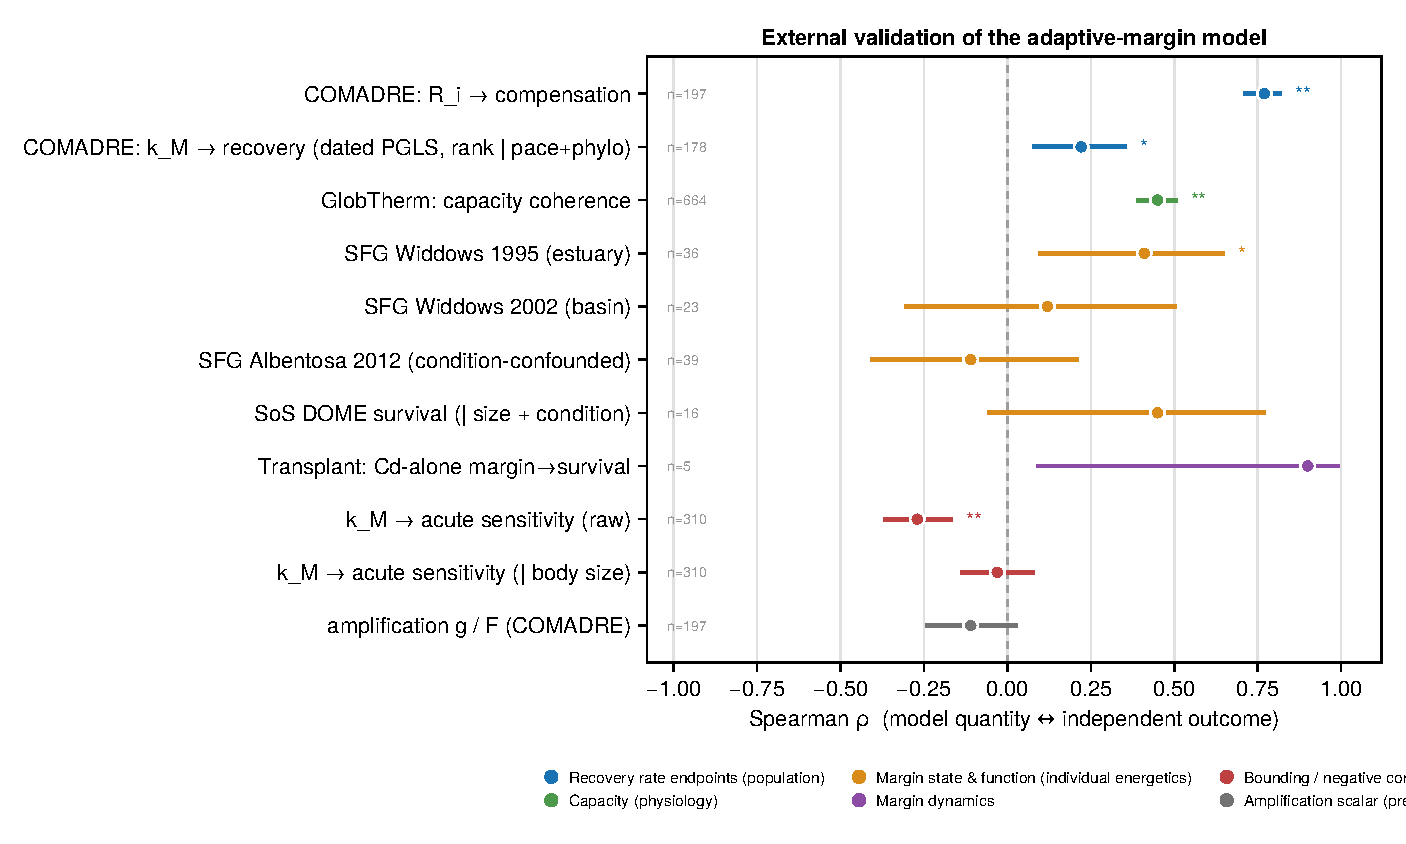
\includegraphics[width=\linewidth]{validation_forest.pdf}
\caption{External-validation forest plot. Per-anchor Spearman $\rho$ (point) with Fisher-$z$
approximate 95\% confidence intervals (bars), grouped by organisational level. Positive $\rho$ indicates
the model quantity tracks the independently measured outcome in the pre-registered direction. The
positive cluster (recovery endpoints, margin state/function, dynamics) contrasts with the
\emph{bounding} negative controls --- $k_M\to$acute sensitivity is non-trivial raw but collapses under
a body-size control ($n{=}310$) --- and the amplification scalar $g/\mathcal{F}$, which is null as the
margin-first reading predicts. CIs are illustrative (some anchors are small-$n$ or figure-digitised);
$^{*}p<0.05$, $^{**}p<0.01$.}
\label{fig:forest}
\end{figure}

\section{Discussion}
\label{sec:discussion}

External evidence supports the \textbf{margin/recovery layer} at four organisational levels --- its
rate endpoints, its state, its function, and a first sign of its dynamics (Figure~\ref{fig:forest}) ---
while the amplification scalar is null throughout, exactly as the margin-first reframe predicts. Three honest qualifications
define the result.

\paragraph{Rank-robust, magnitude-modest, specification-sensitive.} Effects are $\rho\approx0.2$--$0.45$
--- corroboration, not strong prediction --- and several live in the ranks (the headline $k_M$ result
survives a dated-tree PGLS in rank form but nulls in log-linear form). They should be reported as
monotone tendencies.

\paragraph{Tissue burden $\neq$ exposure, and the metals lesson.} The pressure proxy is a relative
tissue burden; where burden tracks food/condition rather than exposure it fails (Albentosa). This is why
metals route to maintenance in field data: it is a \emph{confound-control}, not a mechanistic claim.
Fitted DEBtox modes of action place metals on assimilation, but re-routing metals to assimilation
\emph{degrades every field anchor} (e.g.\ Widdows 1995 ${+}0.41\to{+}0.30$; Widdows 2002
${+}0.12\to{-}0.14$). The two assignments therefore coexist by data regime: field measured burden uses
the maintenance confound-control; controlled or exposure-derived burden may use the fitted assimilation
mode.

\paragraph{The distinctive content is the capacity weighting, and it is carried as an assumption.}
Every individual-level test is single-species, so the AmP capacity weighting is held constant; and the
single-trait $k_M\to$toxicity link is body-size-confounded. The model's distinctive across-axis
capacity weighting therefore remains \emph{untested}, awaiting across-species contaminant-gradient data
that largely does not exist; it is stated as a model assumption, like the mixture rules.

\paragraph{Scope for water-quality application.} The validated machinery (margin, saturating response,
recovery dynamics) supports \emph{relative}, mechanistically structured vulnerability statements ---
ranking sites and months under sustained pressure --- rather than absolute risk thresholds or
across-species predictions. That is the defensible use the present evidence licenses.

\section*{Reproducibility and data availability}
All anchors use openly available data (COMADRE, GlobTherm, ICES DOME OSPAR CEMP, EPA ECOTOX, AmP) or
published tables; raw downloads are gitignored and derived tables, harnesses, and analysis scripts are
in the repository (\texttt{examples/}, \texttt{scripts/}, \texttt{data/external/}). A consolidated
account with per-anchor detail is \texttt{docs/notes/external\_validation\_synthesis.md}. Statistics are
Spearman rank correlations with pre-registered signs; analyses run under Julia 1.12.6.

\bibliographystyle{plainnat}
\bibliography{validation_refs}

\end{document}
